\chapter{Módulo 1. Matéria e energia}

\coment{BNCC: (EF05CI02), (EF05CI03), (EF05CI04).}

\conteudo{A água presente na superfície do planeta Terra se recicla há milhões de
anos. O ciclo hidrológico da água representa o equilíbrio dessas porções
num movimento contínuo, que acontece por conta das mudanças de estado
físico, e é influenciado pelas movimentações do recurso natural na
natureza ou realizadas pelos seres humanos. Nesse ciclo, a água é
naturalmente reciclada, ao ser evaporada de solos e rios, transpirada
pela vegetação e condensada nas nuvens, para então se precipitar e cair
de volta na superfície sob a forma de chuva. Ele pode ser alterado a
depender da realidade de cada região, dos hábitos da população, da
preservação ambiental e dos fenômenos naturais.

Em algumas situações, o funcionamento do ciclo hidrológico da água é
interrompido por características naturais ou intensificadas pela ação
humana. Problemas com a qualidade dos solos, desmatamento e poluição
atuam na potencialização do assoreamento dos rios, o depósito de
sedimentos no fundo das águas, que pode mudar cursos d'água, causar
inundações ou mesmo inviabilizar a sobrevivência de espécies marinhas.

Para garantir a preservação das condições ambientais, deve-se atentar
para os usos conscientes da água, tanto em atividades comuns do
dia-a-dia, como escovar os dentes, tomar banho e lavar calçadas, quanto
em observar os usos do recurso natural na produção agrícola e industrial
de larga escala.}

\colorsec{Atividades}

\num{1} Indique, nos retângulos vazios, o nome das mudanças de
estado físico no ciclo hidrológico da água.

%ILUSTRAÇÃO SIMPLES INDICANDO O CICLO HIDROLÓGICO DA ÁGUA, CONTENDO UM SOLO GRAMADO, COM PELO MENOS UMA ÁRVORE, AO LADO DE UM OCEANO/RIO/LAGO. EXPLICITAR, NO CÉU, O SOL AO LADO DE NUVENS.

%SETAS SAEM DO OCEANO E DA ÁRVORE, E VÃO NA DIREÇÃO DO CÉU, CHEGANDO ATÉ AS NUVENS.

%SETAS SAEM DAS NUVENS ATÉ OUTRAS NUVENS, INDICANDO CHUVA; IMPORTANTE QUE AS ``OUTRAS NUVENS'' ESTEJAM NUM NÍVEL ABAIXO DAS ANTERIORES, E EM TONALIDADE MAIS ESCURA INDICANDO QUE ESTÃO ``CHEIAS'' DE ÁGUA. NA ÁRVORE, NO OCEANO E NAS NUVENS, INSERIR RETÂNGULOS VAZIOS PARA QUE OS ALUNOS COMPLETEM COM O NOME DO FENÔMENO. SE POSSÍVEL, INDICAR ABAIXO DO GRAMADO UM ESPAÇO MARROM, O SUBSOLO, COM UM CAMINHO DE ÁGUAS SUBTERRÂNEAS QUE SE CONECTAM AO OCEANO.

\coment{Eixo A, (EF05CI02) O calor gerado pelos raios solares aquece a água dos
oceanos e a água armazenada nos solos, evaporando-a (evaporação), além
de atuar na transpiração das árvores que absorvem a água do solo
(transpiração ou evapotranspiração). As nuvens se carregam dos vapores
d'água (condensação), até que as gotículas se agregam e caem na
superfície terrestre (precipitação).}

\num{2} Relacione as colunas, indicando o uso da água de acordo com
a atividade correspondente.

\begin{multicols}{2}
\red{Irrigação}

\red{Limpeza de casa}

\red{Produção de energia}

\red{Extração mineral}

\blue{Uso doméstico}

\blue{Termeletricidade}

\blue{Mineração}

\blue{Agricultura}

\end{multicols}

\coment{Eixo A, (EF05CI02) Relações: Irrigação-Agricultura; Limpeza de casa-Uso
doméstico; Produção de energia-Termeletricidade; Extração
mineral-Mineração.}

\num{3} Leia o texto

\begin{quote}
Em todo o país, pouco menos da metade das escolas públicas (46,7\%) têm
acesso a saneamento básico - isso significa distribuição de água
potável, coleta e tratamento de esgoto, drenagem urbana e coleta de
resíduos sólidos.

\fonte{TOKARNIA, Mariana. \textbf{Quase metade das escolas não tem todos os
itens de saneamento básico}. Disponível em:
https://agenciabrasil.ebc.com.br/educacao/noticia/2020-06/quase-metade-das-escolas-nao-tem-todos-os-itens-de-saneamento-basico.
Acesso em: 13 fev. 2023.}
\end{quote}

Como a falta do serviço mencionado no texto afeta, além das escolas, a
vida da população?

\linhas{3}

\coment{Eixo B, (EF05CI02) O serviço mencionado é o saneamento básico. As
consequências da falta desse serviço são variadas, como na propagação de
doenças a partir de uma rede de esgoto não tratada, poluição urbana,
agravamento de desigualdades sociais, aumento da mortalidade,
desequilíbrio de ecossistemas, falta de higiene pessoal, infestação de
pragas, acúmulo de lixo, enchentes, contaminação de lençóis freáticos,
dentre outras problemáticas.}

\num{4} Crises hídricas no espaço urbano consistem na interrupção
do fornecimento de água tratada para a população. Elas ocorrem,
principalmente, por conta da diminuição do nível de reservatórios, em
épocas com volume de chuva escasso.

É comum observar, nestas situações, soluções alternativas da população
para lidar com a falta d'água, como recolher a água da chuva, carregar
baldes de rios e lagos e racionar a água disponível na caixa d'água.

\begin{escolha}
\item A água da chuva é potável, isto é, própria para o consumo
humano?

\linhas{3}

\coment{Eixo B, (EF05CI02) Não. A água da chuva é contaminada por substâncias
tóxicas para os seres humanos, presentes na atmosfera, além de conter
microrganismos como bactérias. O consumo humano dessa fonte de água pode
levar a intoxicações e doenças.}

\item Se a quantidade de água do planeta se mantém constante há
milhões de anos, como pode ocorrer a falta deste recurso para as
populações humanas?

\linhas{3}

\coment{Eixo C, (EF05CI02) O planeta Terra possui água em abundância, mas apenas
uma pequena parte (0,02\%) é de fácil acesso e própria para o consumo.
As proporções de água se mantêm constantes há milhões de anos, porém, a
quantidade de água de qualidade não. Fenômenos naturais e humanos podem
alterar essas proporções, principalmente quando há mudanças climáticas
que impactam no ciclo hidrológico, ou mesmo poluição.}
\end{escolha}

\num{5}

O assoreamento é um processo de alteração dos cursos
d'água de oceanos e rios a partir da elevação do seu leito, pelo acúmulo
de sedimentos. Apesar de natural, é potencializado pela ação humana, e
dificulta a navegação, ocasiona cheias e inundações, além da perda de
vegetação subaquática e alteração do habitat de animais marinhos.

Marque a alternativa que representa uma causa da intensificação do
assoreamento.

\begin{escolha}
\item Falta de chuvas.

\item Remoção da mata ciliar.

\item Contaminação da água.

\item Uso de navios.
\end{escolha}

\coment{Eixo B, (EF05CI03) Letra b. Uma das causas da intensificação do
assoreamento é a remoção da mata ciliar, ou seja, a vegetação presente
em locais próximos aos corpos de água. Essa mata é responsável por
conter o acúmulo de detritos sólidos no fundo dos rios, e, quando
removida pela ação humana, contribui para potencializar a ocorrência do
assoreamento.}

\num{6} Marque verdadeiro (\salmao{V}) ou falso (\salmao{F}):

\begin{boxlist}
\item A cobertura vegetal regula o ciclo hidrológico da água ao reduzir 
a erosão e o assoreamento, além de diminuir o risco de inundações. \coment{V}

\item A erosão é um processo natural de desgaste de solos e rochas, e 
não pode ser agravado pela atividade humana. \coment{F}

\item A presença de vegetação melhora a qualidade do solo, que contém 
reservas de água e de nutrientes para as plantas. \coment{V}

\item O ar atmosférico se torna mais puro em áreas com ampla presença de 
vegetação, que atua para filtrar os contaminantes. \coment{V}
\end{boxlist}

\coment{Eixo B, (EF05CI03) Ordem das respostas: V, F, V, V. A alternativa falsa
descreve o processo natural da erosão corretamente, mas descarta a
influência da atividade humana, capaz de potencializá-lo. Discuta com os
alunos as possibilidades biológicas, químicas e geográficas de
potencialização do processo de erosão, desde a incorreta destinação de
rejeitos industriais, desmatamento, queimadas, uso excessivo de
fertilizantes, até a contaminação da atmosfera e, consequentemente,
toxicidade da chuva.}

\num{7} Leia o texto:

\begin{quote}
Além das mortes, desastres ambientais causam prejuízos materiais e
formam uma multidão de famílias sem ter onde morar. Conforme o
\textbf{Atlas Digital de Desastres no Brasil}, houve 18.551 ocorrências
de inundações, enchentes, enxurradas e deslizamentos entre os anos de
1995 e 2019, resultando em 6,629 milhões de desabrigados e desalojados e
67,516 milhões de pessoas afetadas. Já os danos materiais são calculados
em R\$59,360 bilhões, em valores corrigidos. Se considerar outros
desastres, como incêndios florestais, os prejuízos são ainda maiores.

\fonte{MENGUE, et. al. \textbf{Brasil tem quase 4 mil mortes por deslizamentos
de terra}. Disponível em:
https://www.terra.com.br/noticias/brasil/cidades/brasil-tem-quase-4-mil-mortes-por-deslizamentos-de-terra,43b8e0c71f1d32c1a69b88fbcc4b0ede40xtezym.html.
Acesso em: 14 fev. 2023.}
\end{quote}

Como consequência direta de fortes chuvas, deslizamentos de terra são
frequentes e causam danos materiais e sociais profundos quando ocorrem.
Esses fenômenos, no entanto, poderiam ser evitados com a preservação da
vegetação no entorno de encostas, morros e serras.

Qual o papel da cobertura vegetal em evitar desastres como os
deslizamentos de terra?

\linhas{4}

\coment{Eixo C, (EF05CI03) A cobertura vegetal, quando preservada, pode
funcionar como barreira para o arraste de sedimentos pela chuva,
evitando ou reduzindo os impactos de um deslizamento de terra,
principalmente em locais íngremes, morros e serras. Além disso, a
preservação do solo é primordial para que parte da água da chuva seja
absorvida.}

\num{8} Ao realizar colheitas de safras de café, um fazendeiro
notou que a qualidade do solo empobreceu no decorrer dos anos,
totalizando grandes perdas por efeitos naturais causados pelo vento e a
chuva, e infestação de pragas. Ao pesquisar sobre formas de combater o
processo de erosão observado, ele chegou às seguintes opções:

\begin{tabular}{|l|l|l|}
\hline
\textbf{Ação} & \textbf{Custo} & \textbf{Tempo/Condições} \\ \hline
\begin{tabular}[c]{@{}l@{}}1 - Plantar vegetais como\\ eucalipto e cana-de-açúcar\\ ao redor da lavoura, para\\ protegê-la da erosão eólica\\ e pluvial, além de inserir\\ insetos predadores para\\ eliminar as pragas.\end{tabular} & Baixo & \begin{tabular}[c]{@{}l@{}}O resultado só poderá ser\\ avaliado dentro de alguns\\ meses, mas diminuirá\\ significativamente o\\ processo erosivo.\end{tabular} \\ \hline
\begin{tabular}[c]{@{}l@{}}2- Plantar somente em\\ curvas de nível, para\\ limitar a velocidade e\\ evitar que a água da\\ chuva provoque a erosão.\end{tabular} & Alto & \begin{tabular}[c]{@{}l@{}}O resultado aparece em\\ algumas semanas, pois\\ exige grandes adaptações\\ no formato de toda a\\ lavoura e diminui a\\ capacidade produtiva.\end{tabular} \\ \hline
\begin{tabular}[c]{@{}l@{}}3- Usar, além de barreiras\\ de contenção de madeira e\\ concreto, substâncias para\\ controlar a proliferação\\ de pragas, os chamados\\ defensivos agrícolas.\end{tabular} & Baixo & \begin{tabular}[c]{@{}l@{}}O resultado é rápido. As\\ contenções podem atuar\\ assim que forem\\ construídas, mas o\\ concreto agride o solo\\ ao redor da lavoura e os\\ defensivos agrícolas podem\\ conter componentes tóxicos.\end{tabular} \\ \hline
\end{tabular}

O fazendeiro pode escolher qualquer uma das opções, ou combiná-las, se
necessário. Qual a melhor escolha, observando os ganhos para a produção
e a preservação do solo?

\linhas{5}

\coment{Eixo C, (EF05CI03) As opções 1 e 2 são as melhores escolhas, pois
garantem soluções diretas para os principais problemas que acometem a
lavoura, sem deixar de observar que a preservação do ambiente é
importante para as cadeias produtivas, além de se levar em conta que,
mesmo com as limitações produtivas de tempo, à longo prazo essas medidas
são mais benéficas ao solo. A opção 3, apesar de ser barata e rápida,
agride o ambiente, pode acelerar o processo erosivo em outras frentes e
ainda expõe o produto aos efeitos de um agente tóxico, representando uma
solução imediatista.}

\num{9} Apesar de não-potável, a água da chuva pode ser reutilizada
em atividades em que o gasto de água limpa é excessivo. A principal
recomendação é que se descarte a primeira porção de água da chuva
recolhida, pois nela estão concentradas as maiores quantidades de
impurezas.

Descreva duas situações cotidianas para a reutilização não-potável da
água.

\linhas{4}

\coment{Eixo C, (EF05CI04) O uso não-potável da água deve ser abordado
principalmente em atividades em que o gasto de água potável é excessivo.
A água da chuva pode ser reaproveitada em atividades como a lavagem de
calçadas e superfícies, costumeiramente realizada com mangueiras. Além
disso, não há problema em reutilizar a água da chuva para a irrigação de
plantas e demais tipos de vegetação.}

\num{10} O consumo consciente da água deve ser, segundo a ONU, de
110 litros em média per capita. Isso significa dizer que, no decorrer de
um dia, devem-se observar as atividades que desperdiçam água em excesso.
A tabela abaixo traz informações sobre algumas dessas atividades:

\begin{tabular}{|l|l|}
\hline
\textbf{Atividade} & \textbf{Consumo de água} \\ \hline
Escovar os dentes & \begin{tabular}[c]{@{}l@{}}Torneira aberta: 18 litros\\ Abrindo e fechando a torneira: 2 litros\end{tabular} \\ \hline
Banho & \begin{tabular}[c]{@{}l@{}}20 minutos: 120 litros\\ 5 minutos: 30 litros\end{tabular} \\ \hline
Lavar a calçada & Em média 120 litros \\ \hline
Torneiras pingando & \begin{tabular}[c]{@{}l@{}}Gotas de água: 48 litros\\ Água em filetes: 180 a 750 litros\end{tabular} \\ \hline
Lavar a louça & \begin{tabular}[c]{@{}l@{}}Água aberta continuamente: 240 litros\\ Abrindo e fechando a torneira: 70 litros\end{tabular} \\ \hline
\end{tabular}

\fonte{Fonte: CAESB
(https://www.caesb.df.gov.br/dicas-consumo-agua.html)}

Para se adequar à recomendação da ONU, uma pessoa deve escolher quais
atividades e qual modelo de consumo de água?

\linhas{4}

\coment{Eixo C, (EF05CI04) Para se adequar até a média de 110 litros de consumo,
uma pessoa deve optar por escovar os dentes abrindo e fechando a
torneira, tomar banhos de até 5 minutos, e lavar a louça abrindo e
fechando a torneira, totalizando cerca de 102 litros gastos por dia.
Além disso, não se deve desperdiçar água lavando calçadas, e também
deve-se atentar para vazamentos em torneiras e consertá-los o quanto
antes, pois mesmo o gotejamento pode gastar uma grande quantidade de
água.}

\num{11} O consumo de água na produção de alguns itens não é
verificado diretamente, por isso, chama-se de água invisível ou virtual
a quantidade gasta em processos como a produção de alimentos e
industrial. Segundo estimativas, produzir 1kg de carne bovina consome,
em média, 15.000 litros de água, enquanto a produção de um smartphone
pode consumir 12.600 litros de água, o equivalente à capacidade de um
caminhão-pipa.

\begin{escolha}
\item Cite formas de economizar água invisível.

\linhas{4}

\coment{Eixo B, (EF05CI04) Nos casos citados, a água invisível pode ser
economizada ao reduzir o consumo de carnes vermelhas e preservar objetos
como smartphones, evitando as trocas desnecessárias. Esse tipo de
consumo também se apresenta na produção de alimentos variados,
cosméticos, roupas, carros. Debata com a turma outras formas de
utilização da água invisível e oriente uma pesquisa sobre outros bens do
cotidiano que possam utilizar desse recurso.}

\item Em processos industriais, a água é consumida em grandes
volumes. O que é necessário fazer caso se deseje devolver águas
residuais para o meio ambiente?

\linhas{4}

\coment{Eixo C, (EF05CI04) As águas residuais devem ser sempre tratadas antes de
serem devolvidas ao meio ambiente ou reutilizadas de maneira a entrarem
no ciclo hidrológico da água. O tratamento se dá de diversas maneiras,
objetivando-se a remoção de impurezas, componentes tóxicos e
microrganismos da água residual.}
\end{escolha}

\colorsec{Treino}

\num{1} A Amazônia é um bioma de floresta tropical, e além da
cobertura no noroeste do Brasil, se estende para países como Bolívia,
Colômbia, Equador, Peru e Venezuela. Uma das características mais
marcantes da região é a elevada umidade do ar, consequência da ação de
árvores que absorvem a água dos solos e transportam-na até as folhas. É
comum, em locais da região Norte do Brasil, a ocorrência de chuvas
diariamente.

O fenômeno descrito no texto é chamado de

\begin{escolha}
\item ebulição.

\item evapotranspiração.

\item condensação.

\item precipitação.
\end{escolha}

\coment{Saeb: Eixo cognitivo A.

BNCC: (EF05CI02) Aplicar os conhecimentos sobre as mudanças de estado
físico da água para explicar o ciclo hidrológico e analisar suas
implicações na agricultura, no clima, na geração de energia elétrica, no
provimento de água potável e no equilíbrio dos ecossistemas regionais
(ou locais).

a) Incorreto. A ebulição é a passagem rápida de uma substância do estado
líquido para o estado gasoso em determinada temperatura. No caso
mencionado, há um fenômeno específico realizado em condições próprias de
solo e vegetação, como na floresta amazônica, chamado de
evapotranspiração;
b) Correto. A evapotranspiração é um fenômeno que combina a evaporação
de líquidos com a transpiração de folhas. No caso da floresta amazônica,
a umidade se eleva pois as árvores funcionam como ``bombas'' de água,
participando também da regulação do regime de chuvas de toda a região;
c) Incorreto. A condensação ocorre quando há a agregação de substâncias
gasosas, de modo que as partículas se unam e formem um líquido. Esse
fenômeno pode acontecer nas nuvens, numa das etapas do ciclo hidrológico
da água, mas não é descrito no texto;
d) Incorreto. A precipitação ocorre quando há quantidade suficiente de
água no estado líquido nas nuvens, e então, chove. Apesar da chuva ser
mencionada no texto, não há descrição desse fenômeno, e sim da
evapotranspiração, processo em que a combinação de evaporação da água de
solos e transpiração das folhas acontece.}

\num{2}

\begin{quote}
Os mapas e dados atualizados do MapBiomas mostram que o Brasil perdeu
87,2 milhões de hectares de áreas de vegetação nativa, de 1985 a 2019.
Isso equivale a 10,25\% do território nacional. O ritmo de perda de
vegetação nativa acelerou no Brasil entre 2018 e 2019.

\fonte{BRASIL perdeu 10\% do território em vegetação nativa entre 1985 e 2019.
Disponível em:
https://ipam.org.br/brasil-perdeu-area-de-vegetacao-nativa-equivalente-a-10-do-territorio-nacional-entre-1985-e-2019/.
Acesso em: 14 fev. 2023.}
\end{quote}

As consequências desse problema podem resultar na

\begin{escolha}
\item regulação do regime de chuvas.

\item eliminação de poluentes das florestas.

\item diminuição das reservas de água.

\item erosão de solos e inundação de rios.
\end{escolha}

\coment{Saeb: Eixo cognitivo B.

BNCC: (EF05CI03) Selecionar argumentos que justifiquem a importância da
cobertura vegetal para a manutenção do ciclo da água, a conservação dos
solos, dos cursos de água e da qualidade do ar atmosférico.

a) Incorreto. A perda de vegetação acentua a desregulação do regime de
chuvas, pois desequilibra o ciclo hidrológico da água;
b) Incorreto. O problema mencionado é a diminuição da cobertura vegetal,
logo, não há relação com a eliminação de poluentes das florestas, que
pode se dar a partir de iniciativas para localizar os focos de poluição
e realizar forças-tarefa para preservar o ambiente;
c) Incorreto. A redução da cobertura vegetal pode acarretar no
desequilíbrio do ciclo hidrológico da água, e favorece o acontecimento
de fenômeno como o assoreamento, que altera os cursos d'água e eleva o
leito de rios e lagos;
d) Correto. A perda de vegetação pode acarretar num extenso processo de
erosão dos solos que tem como uma das principais consequências a
inundação de rios, causada por fenômenos como o assoreamento, quando a
falta de vegetação aliada com a perda da qualidade do solo faz com que
detritos sólidos sejam arrastados para o fundo dos rios, elevando o
leito.}

\num{3} Operários de um conglomerado industrial perceberam que, ao
fim da produção de alimentos, as quantidades residuais de água eram
despejadas para o esgoto, e que, para a higienização das superfícies
internas e externas, bombeava-se uma grande quantidade de água potável.
Pensando nisso, elaboraram um material estimativo comparando as
atividades, de forma a reduzir o gasto de água potável e reaproveitar a
água residual. Eles organizaram as informações numa tabela:

\begin{tabular}{|l|l|l|}
\hline
\textbf{Atividade} & \textbf{Uso} & \textbf{Economia} \\ \hline
\begin{tabular}[c]{@{}l@{}}Reaproveitamento da água\\ residual em todos os\\ processos, e\\ armazenamento em tanques.\end{tabular} & \begin{tabular}[c]{@{}l@{}}Limpeza das superfícies da\\ fábrica com o uso de uma\\ bomba, refrigeração e\\ geração de energia.\end{tabular} & 70\% da água potável gasta. \\ \hline
\end{tabular}

Impressionados com as possibilidades de reuso da água, os chefes
ordenaram que todas as atividades calculassem os percentuais de resíduos
aptos para o reuso, interessados em criar um ciclo hidrológico dentro da
indústria. Contudo, foram advertidos de que nem todos os usos poderiam
ser estimulados, exigindo maiores adaptações para fins potáveis.

As advertências foram necessárias pois

\begin{escolha}
\item a água residual pode contaminar as superfícies metálicas.

\item o descarte de água residual no meio ambiente não contamina os mananciais.

\item a água reutilizada para o consumo humano deve ser tratada adequadamente.

\item o reaproveitamento da água traz poucos benefícios.
\end{escolha}

\coment{Saeb: Eixo cognitivo C.

BNCC: (EF05CI04) Identificar os principais usos da água e de outros
materiais nas atividades cotidianas para discutir e propor formas
sustentáveis de utilização desses recursos.

a) Incorreto. A água residual, desde que não tenha componentes
corrosivos, não deve ser contaminante das superfícies metálicas a serem
lavadas. Em muitas situações, ela pode ser reaproveitada em atividades
como lavagens, irrigação de plantas e descarga de bacias sanitárias;
b) Incorreto. A água residual não-tratada pode contaminar os mananciais
de água limpa, sem passar pelo tratamento adequado. Caso se deseje
devolver a água para os mananciais, deve-se adotar um regime de
tratamento avançado para eliminar microrganismos e componentes tóxicos
da água residual;
c) Correto. Caso se deseje reutilizar água residual para fins potáveis,
deve-se adotar um esquema avançado de tratamento a fim de filtrar as
impurezas e eliminar microrganismos da água, além de propor uma
avaliação da qualidade para o consumo humano;
d) Incorreto. O reaproveitamento da água traz grandes benefícios em
termos de economia de recursos e do uso sustentável de um bem natural.
Ele pode ser realizado em escala doméstica, reaproveitando água para
procedimentos como lavagens de calçadas e carros, ou em escala
industrial, com a reutilização de água residual em processos de lavagem
e produção de energia.}

\chapter{Módulo 2. vida e evolução}

\coment{BNCC: (EF05CI06), (EF05CI07), (EF05CI08).}

\conteudo{O corpo humano possui diversos órgãos que funcionam em sistemas. O
sistema digestório é responsável pelas etapas de digestão dos alimentos,
processo que se inicia na boca e termina no intestino grosso. É nesse
sistema que acontecem as divisões dos alimentos em porções menores,
absorção de diferentes tipos de nutrientes nos órgãos e separação e
eliminação das sobras. A ação do sistema digestório é essencial para a
nutrição do organismo e produção de energia.

No sistema respiratório, num circuito desde as fossas nasais até as
estruturas do pulmão, ocorre a inspiração de gás oxigênio e expiração de
gás carbônico. Enquanto o gás oxigênio é incorporado ao sangue, o gás
carbônico, produto de processos energéticos do organismo humano, é
eliminado. Nesse sistema, há o provimento de oxigênio que será utilizado
nos processos de divisão dos alimentos, gerando energia.

O transporte de oxigênio e de nutrientes é realizado pelo sistema
circulatório, que incorpora essas substâncias na corrente sanguínea,
transportada pelas veias e artérias e bombeadas para todas as partes do
corpo pelo coração. A atuação em conjunto com outros sistemas garante
que os tecidos do corpo humano serão nutridos após a alimentação.

O funcionamento regular dos sistemas depende da alimentação saudável em
boas fontes de nutrientes. Alimentos com quantidades balanceadas de
carboidratos e gorduras, e ricos em fibras, proteínas e vitaminas são
essenciais para garantir que o máximo de nutrientes será absorvido pelo
organismo, enquanto alimentos com calorias baseadas no excesso de
carboidratos e gorduras podem fazer com que o organismo se torne
deficiente em nutrientes e armazene gordura.}

\colorsec{Atividades}

\num{1} Complete o texto com as palavras disponíveis.

\begin{itemize}
\item Boca

\item Estômago

\item Saliva

\item Esôfago

\item Quilo

\item Intestino delgado

\item Quimo

\item Intestino grosso

\item Fezes

\item Suco gástrico.
\end{itemize}

\begin{quote}
A digestão começa na \preencher\coment{boca}, onde os alimentos ingeridos são
triturados e envolvidos pela \preencher\coment{saliva}, responsável por digerir
o amido. O alimento é engolido, e passa pelo \preencher\coment{esôfago}, que faz
movimentos peristálticos para empurrá-lo até o \preencher\coment{estômago}.
Depois, o alimento é amassado e se mistura com o \preencher\coment{suco gástrico}.

Alguns nutrientes são absorvidos no estômago, enquanto o resto do bolo
alimentar, chamado de \preencher\coment{quimo} segue para o \preencher\coment{intestino delgado}. Lá, parte dos nutrientes é aproveitada para a produção de
energia, e o restante passa a ser chamado de \preencher\coment{quilo}. No \preencher\coment{intestino grosso} a água e os nutrientes restantes são levados para o
organismo, e a sobra é eliminada no formato de \preencher\coment{fezes} pelo
ânus.
\end{quote}

\coment{Eixo A, (EF05CI06)}

\num{2} O corpo humano precisa de energia para funcionar, e ela é
produzida com a junção de sistemas do organismo. Um desses sistemas, o
digestório, é responsável por processar os alimentos depois da ingestão.

\begin{escolha}
\item Como a alimentação participa da produção de energia para o corpo humano?

\linhas{2}

\coment{Eixo A, (EF05CI06) A partir da alimentação, são absorvidos nutrientes
essenciais para a produção de energia pelo corpo humano, como proteínas,
fibras, vitaminas e gorduras.}

\item Como os bebês, apesar de não terem dentes, conseguem energia para
sobreviver?

\linhas{3}

\coment{Eixo A, (EF05CI06) O aleitamento materno garante a nutrição dos bebês
por conter água e todos os nutrientes necessários para o desenvolvimento
saudável. Como eles não possuem dentes, teriam dificuldades em mastigar
alimentos maiores.}
\end{escolha}

\num{3} Observe a imagem e responda.

\begin{figure}[htpb!]
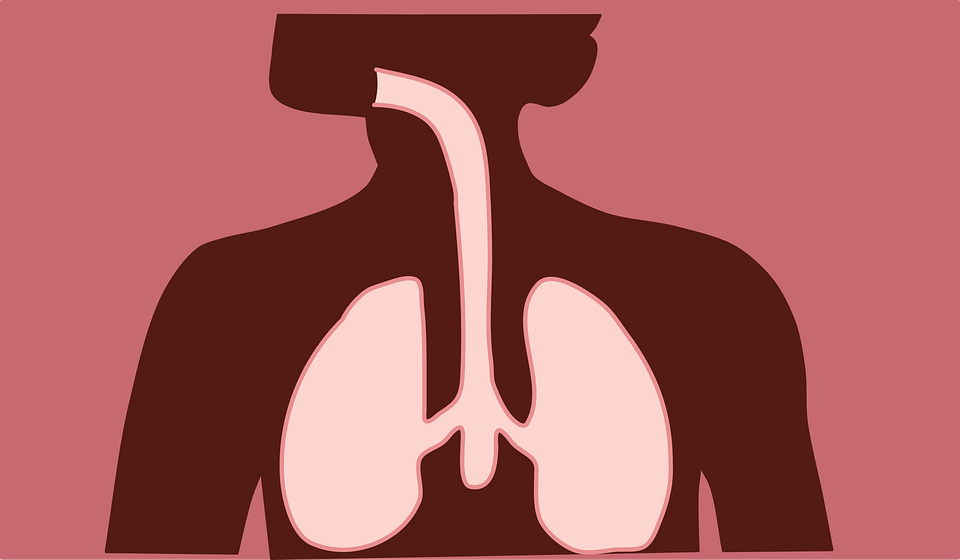
\includegraphics[width=\textwidth]{./imgs/img1.png}
\end{figure}
\fonte{\emph{https://pixabay.com/pt/vectors/sistema-respirat\%c3\%b3rio-respirat\%c3\%b3rio-4869736/}}

\begin{escolha}
\item Quais são os órgãos representados na imagem?

\linhas{1}

\coment{Eixo A, (EF05CI06) Os pulmões.}

\item Esses órgãos são os únicos responsáveis pela respiração humana?

\linhas{2}

\coment{Eixo B, (EF05CI06) Não, além dos pulmões, participam da respiração as
fossas nasais, faringe, traquéia, brônquios, bronquíolos, e alvéolos.}
\end{escolha}

\num{4} Durante a respiração, são realizados movimentos pelos
pulmões. Num deles, o nariz puxa o oxigênio do ar, os pulmões enchem e
ficam inflados, como um balão. Depois, esvaziam, com a liberação de gás
carbônico para o meio ambiente pelo nariz ou pela boca.

Como são chamados esses movimentos?

\linhas{1}
\coment{Eixo A, (EF05CI06) Inspiração e Expiração.}

\num{5} Complete a tabela com as informações corretas

\begin{tabular}{|l|l|l|}
\hline
\textbf{Processo} & \textbf{O que ocorre?} & \textbf{Onde ocorre?} \\ \hline
Troca gasosa & \begin{tabular}[c]{@{}l@{}}O oxigênio presente no ar\\ é inspirado e levado até\\ a corrente sanguínea,\\ enquanto o gás carbônico\\ é liberado via expiração\end{tabular} & \rosa{Pulmões} \\ \hline
Circulação sanguínea & \begin{tabular}[c]{@{}l@{}}\rosa{O sangue, concentrado em}\\ \rosa{oxigênio e nutrientes, é}\\ \rosa{bombeado para todas as}\\ \rosa{extremidades do corpo}\end{tabular} & \begin{tabular}[c]{@{}l@{}}Coração e\\ \rosa{vasos sanguíneos}\end{tabular} \\ \hline
\begin{tabular}[c]{@{}l@{}}Transporte de nutrientes,\\ como a glicose, para a célula\end{tabular} & \begin{tabular}[c]{@{}l@{}}\rosa{Os nutrientes são levados a}\\ \rosa{todos órgãos, assim é gerada}\\ \rosa{energia ou se formam}\\ \rosa{reservas de gordura}\end{tabular} & No sistema circulatório \\ \hline
\end{tabular}

\coment{Eixo B, (EF05CI06); (EF05CI07)}

\num{6} Marque verdadeiro (V) ou falso (F):

\begin{boxlist}
\item Fazem parte do sistema circulatório o sangue, os vasos sanguíneos e o coração. \coment{V}

\item O sangue percorre todo o organismo, mas somente os pulmões transportam oxigênio. \coment{F}

\item O coração bombeia o sangue para todas as extremidades do corpo humano. \coment{V}

\item Os vasos sanguíneos podem se dilatar em temperaturas muito baixas. \coment{F}

\item Quando praticamos atividades físicas, o coração bombeia mais rápido 
o sangue contendo nutrientes e oxigênio por todo o organismo. \coment{V}
\end{boxlist}

\coment{Eixo B, (EF05CI07) V, F, V, F, V. Primeira alternativa falsa: O sangue
transporta oxigênio por todo o organismo, e não os pulmões. Segunda
alternativa falsa: Os vasos sanguíneos se contraem em temperaturas muito
baixas, e dilatam novamente com o aumento de temperatura.}

\num{7} Quando o corpo humano entra em contato com alguma doença, e
desenvolve uma infecção, uma defesa é produzida, e depois transportada
pelo sangue para combater o efeito das células malignas.

\begin{escolha}
\item Como são chamadas as células defensivas?

\linhas{1}

\coment{Eixo A, (EF05CI07) As células de defesa capazes de combater uma infecção
são chamadas de anticorpos.}

\item Como essas células atuam?

\linhas{2}

\coment{Eixo B, (EF05CI07) Os anticorpos são liberados na corrente sanguínea
pelo sistema imune após a detecção de um invasor pelos macrófagos, e
atuam cercando as células malignas, destruindo-as.}

\item Qual a importância da vacinação para a produção de defesas do organismo?

\linhas{3}

\coment{Eixo C, (EF05CI07) As vacinas estimulam a liberação de anticorpos para
combater uma infecção bem mais fraca, incapaz de deixar uma pessoa
doente. Mas, como o organismo possui memória imunológica, quando uma
infecção verdadeira ocorrer, os anticorpos estarão presentes e prontos
para combatê-la.}
\end{escolha}

\num{8} Marque a alternativa que descreve as funções do sistema circulatório corretamente.

\begin{escolha}
\item transporte de sangue por todas as extremidades do corpo, contendo
oxigênio, nutrientes e separação de toxinas para eliminação.

\item filtragem de alimentos e do oxigênio respirado, e produção de gás
carbônico para expiração.

\item limpeza das impurezas do organismo, produção do suco gástrico e
remoção de células malignas do corpo.

\item regulagem das fezes produzidas pelo intestino grosso, separando
componentes a serem eliminados.
\end{escolha}

\coment{Eixo C, (EF05CI07) Alternativa a. A descrição das funções do sistema
circulatório abarca o transporte de sangue por todo o corpo, contendo
oxigênio e nutrientes, além da separação de toxinas a serem excretadas.
Dessa maneira, o sistema circulatório se integra ao sistema respiratório
e digestório. As demais alternativas apresentam erros, como em b, ou
informações incompletas e funções indiretas do sistema respiratório,
como em c e d. Discuta com a turma a análise das alternativas
incorretas.}

\num{9} A glicose é um dos principais nutrientes utilizados como
fonte de energia pelos seres humanos. Ela é aproveitada ao ser dividida
e convertida em outras substâncias para produção de energia. Entretanto,
algumas pessoas sofrem com o excesso da presença desse nutriente no
sangue.

Cite uma doença relacionada com o excesso de glicose na corrente
sanguínea.

\linhas{3}

\coment{Eixo A, (EF05CI07) A doença relacionada com o excesso de glicose no
sangue é o diabetes mellitus. Discuta com os alunos sobre experiências
com esse nome, e explique que ela ocorre por conta da falha no organismo
em produzir a substância capaz de dividir ou quebrar a glicose.}

\num{10} A figura a seguir representa um exemplo de pirâmide
alimentar:

\begin{figure}[htpb!]
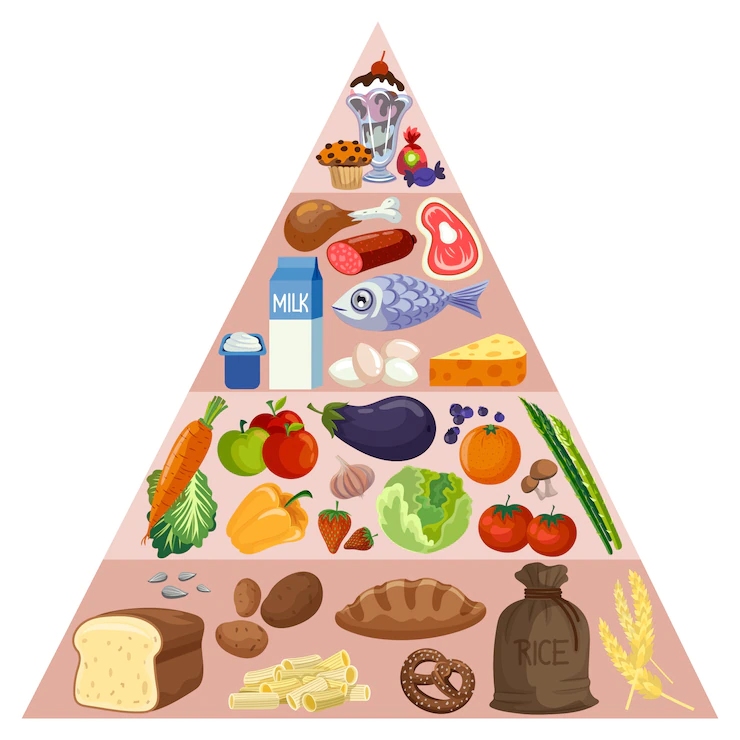
\includegraphics[width=\textwidth]{./imgs/img2.png}
\end{figure}

\fonte{Imagem: Freepik / \emph{https://br.freepik.com/vetores-gratis/conceito-de-nutricao-de-design-de-piramide-alimentar\_7371729.htm\#query=pir\%C3\%A2mide\%20alimentar\&position=1\&from\_view=search\&track=ais}}

Observe a imagem e responda atentamente às perguntas:

\begin{escolha}
\item Por que alguns itens estão na base da pirâmide?

\linhas{3}
\coment{Eixo B, (EF05CI08) Os alimentos da base da pirâmide representam o acesso
às principais fontes de energia para o corpo humano, nutrientes como
carboidratos, de que são ricos os pães, bolos, batatas, grãos, entre
outros.}

\item Por que alguns itens estão no topo da pirâmide?

\linhas{3}
\coment{Eixo B, (EF05CI08) São os alimentos com menor importância para uma
alimentação saudável, e sugestivamente com menor valor nutricional. São
eles os doces, chocolates, frituras e demais alimentos processados.}

\item Qual a recomendação para uma alimentação saudável, observando os alimentos da pirâmide?

\linhas{3}
\coment{Eixo C, (EF05CI08) Observa-se que a alimentação deve ser balanceada, sem
exagerar em nenhuma das etapas da pirâmide, mas composta principalmente
pelos alimentos da base, com participação fundamental, também, de outras
classes representadas, como legumes, laticínios, peixes e carnes (fontes
de proteína).}
\end{escolha}

\num{11} Durante um processo de reeducação alimentar, uma pessoa
estimou que precisava consumir cerca de 1800kcal por dia, resultado
compatível com a sua altura e peso. Para controlar a alimentação, anotou
as informações de alguns alimentos.

\begin{longtable}[]{@{}llllll@{}}
\toprule
\textbf{Alimento (porção de 100g)} & \textbf{Energia (calorias)} &
\textbf{Carboidratos} & \textbf{Gorduras} & \textbf{Proteínas} &
\textbf{Fibra alimentar}\tabularnewline
Batata frita & 250kcal & 33g & 12g & 4g & 3g\tabularnewline
Batata cozida & 50kcal & 12g & 0g & 1g & 1g\tabularnewline
Biscoito doce & 440kcal & 76g & 11g & 8g & 3g\tabularnewline
Banana prata & 105kcal & 26g & 0g & 1g & 2g\tabularnewline
Salada de legumes & 35kcal & 7g & 0g & 2g & 3g\tabularnewline
Pizza calabresa & 260kcal & 33g & 10g & 10g & 2g\tabularnewline
Hambúrguer fast food & 261kcal & 30g & 10g & 13g & 1g\tabularnewline
Risoto de legumes com arroz & 140kcal & 14g & 8g & 3g &
2g\tabularnewline
\bottomrule
\end{longtable}

\fonte{Fonte: Tabela Brasileira de Composição de Alimentos (TBCA).
(Valores adaptados).}

A pessoa notou que, mesmo se a alimentação diária fosse baseada em
alimentos como Batata frita, Biscoito doce, Pizza e Hambúrguer fast
food, não ultrapassaria as necessidades calóricas diárias.

\begin{escolha}
\item Apenas o controle da quantidade de calorias ingeridas é
suficiente para manter uma alimentação saudável?

\linhas{4}
\coment{Eixo C, (EF05CI08) Não, além das calorias ingeridas, a proporção de
nutrientes é fundamental para o equilíbrio da alimentação. Batata frita,
Biscoito doce, Pizza e Hambúrguer fast food são alimentos com grande
quantidade de carboidratos e gorduras, e recomenda-se que não haja
exagero na ingestão desses nutrientes para a manutenção da saúde.}

\item Como uma dieta balanceada deve funcionar?

\linhas{3}
\coment{Eixo C, (EF05CI08) Uma dieta balanceada deve equilibrar o consumo de
carboidratos, gorduras, proteínas e fibras, de acordo com as
necessidades de cada indivíduo. A alimentação com as chamadas calorias
podres, como alimentos ultraprocessados, deve ser reduzida.}

\item Monte, no espaço abaixo, um cardápio para uma alimentação
com base nos alimentos da tabela. Pesquise outros alimentos importantes
para o consumo diário, sem esquecer de anotar as informações
nutricionais.

%Espaço largo em box para que os alunos escrevam o cardápio da forma que preferirem.

\coment{Eixo C, (EF05CI08) Espera-se que os alunos observem as informações
disponíveis em rótulos nutricionais para construir um cardápio
equilibrado, sem exageros ou cortes radicais.}
\end{escolha}

\colorsec{Treino}

\num{1} A alimentação é uma importante fonte de nutrientes para o
corpo humano. Diversos órgãos necessitam da energia gerada a partir da
digestão, onde há a separação do que pode ser aproveitado pelo organismo
e do que deve ser descartado. Os nutrientes, como a glicose e as
proteínas, são levados para todas as extremidades do corpo, e
incorporados aos músculos, estocados na forma de gordura ou degradados.

O transporte dessas substâncias é realizado no

\begin{escolha}
\item sistema circulatório.

\item sistema digestório.

\item sistema respiratório.

\item sistema reprodutivo.
\end{escolha}

\coment{Saeb: Eixo cognitivo A.

BNCC: (EF05CI06) Selecionar argumentos que justifiquem por que os
sistemas digestório e respiratório são considerados corresponsáveis pelo
processo de nutrição do organismo, com base na identificação das funções
desses sistemas.

a) Correto. No sistema circulatório, há o transporte de oxigênio e dos
nutrientes para todas as extremidades do corpo;
b) Incorreto. O sistema digestório é responsável por digerir os
alimentos e separar os nutrientes para o aproveitamento em diferentes
órgãos, e, ao final dele, são descartadas as fezes;
c) Incorreto. No sistema respiratório, há a troca gasosa e o uso do
oxigênio para alguns processos no organismo humano, como na divisão da
glicose em pedaços menores para o transporte. Esse sistema, em si, não
consegue irrigar todas as extremidades do corpo humano;
d) Incorreto. No sistema reprodutivo, acontecem processos relacionados
com a formação e desenvolvimento da vida, e este não é o responsável
pelo transporte de nutrientes para todas as extremidades do corpo.}

\num{2} Segundo dados da Fiocruz e da UNICEF, em 2022 a taxa de
vacinação infantil no Brasil sofreu uma queda brusca, para cerca de
71,49\%. O índice representa um processo acelerado nos últimos anos, em
que a imunização da população infantil caiu da média de 90 a 95\%
registrada nas últimas décadas, aumentando o risco de doenças
erradicadas, ou seja, que tinham desaparecido por conta da vacina,
voltarem a atacar a população.

A falta de vacinação de doenças erradicadas põe uma pessoa em risco pois

\begin{escolha}
\item a estrutura de defesa do corpo só existe com a vacina.

\item a vacina regula sistemas do corpo humano.

\item o organismo fica mais vulnerável a infecções.

\item o sangue precisa levar a vacina para os locais infectados.
\end{escolha}

\coment{Saeb: Eixo cognitivo B.

BNCC: (EF05CI07) Justificar a relação entre o funcionamento do sistema
circulatório, a distribuição dos nutrientes pelo organismo e a
eliminação dos resíduos produzidos.

a) Incorreto. O corpo humano pode produzir células de defesa sozinho,
mas determinadas doenças são muito agressivas e necessitam de defesa
prévia para que o organismo não sofra complicações. Portanto, a
vacinação se faz essencial;
b) Incorreto. O conteúdo da vacina não é capaz de participar da
regulação dos sistemas do organismo, e sim de estimular a produção de
células de defesa pelo sistema imunológico;
c) Correto. Sem a vacinação, as pessoas ficam vulneráveis ao retorno de
doenças por conta da defesa do organismo, que necessita de anticorpos de
memória para combater algumas doenças, e, assim, prevenir casos graves e
mortes;
d) Incorreto. O sangue não leva o conteúdo da vacina para combater
infecções. As vacinas atuam simulando uma infecção mais fraca, para
fazer com que o organismo produza defesas que ficarão na memória
imunológica. Assim, quando a infecção real acontecer, o organismo terá
estruturas para combatê-la.}

\num{3} Leia o texto:

\begin{quote}
No final das contas, as calorias importam, sim, mas nunca sozinhas.
Nosso corpo precisa ser nutrido, algo que algodão doce, batata frita e
outros alimentos ultraprocessados não farão por nós. Eles não estão
proibidos, mas devem ser consumidos com moderação.

\fonte{GARCEZ, Marcella. \textbf{O que a contagem de calorias pode esconder}.
Disponível em:
https://saude.abril.com.br/coluna/com-a-palavra/o-que-a-contagem-de-calorias-pode-esconder/.
Acesso em: 16 fev. 2023.}
\end{quote}

Uma alimentação balanceada deve considerar fatores além da contagem de
calorias, pois

\begin{escolha}
\item as informações dos rótulos nutricionais não são estimativas confiáveis.

\item as necessidades calóricas variam de corpo a corpo.

\item os demais nutrientes, como carboidratos, gorduras e proteínas, devem ser observados.

\item os alimentos ultraprocessados também podem ser benéficos ao organismo.
\end{escolha}

\coment{Saeb: Eixo cognitivo C.

BNCC: (EF05CI08) Organizar um cardápio equilibrado com base nas
características dos grupos alimentares (nutrientes e calorias) e nas
necessidades individuais (atividades realizadas, idade, sexo etc.) para
a manutenção da saúde do organismo.

a) Incorreto. As informações dos rótulos nutricionais estimam a
quantidade de nutrientes do alimento com base no consumo calórico
recomendado diariamente, além de também considerar o consumo médio de
calorias necessárias para o corpo humano, sendo, assim, estimativas
confiáveis;
b) Incorreto. Apesar das necessidades calóricas variarem de corpo a
corpo, o assunto em questão é a contagem de calorias, que não deve ser o
único quesito de avaliação para uma alimentação saudável, visto que dois
alimentos podem apresentar a mesma quantidade calórica numa porção, mas
quantidades diferentes de nutrientes como carboidratos, gorduras e
proteínas;
c) Correto. Demais nutrientes, como carboidratos, gorduras e proteínas
são importantes numa alimentação balanceada. Deve-e evitar o exagero no
consumo de alimentos ricos em gorduras, como os ultraprocessados, pois
eles representam uma fonte pobre de calorias;
d) Incorreto. Os alimentos ultraprocessados representam calorias vazias,
ricas em gorduras e com pouco aproveitamento para o organismo além do
acúmulo de gordura. O consumo em excesso pode, inclusive, ser maléfico à
saúde, causando doenças.}

\chapter{Módulo 3. Terra e Universo}

\coment{BNCC: (EF05CI11), (EF05CI12).}

\conteudo{A Terra é um corpo celeste que faz parte do sistema solar. Em torno do
sol, o planeta realiza movimentos que garantem a manutenção da
sobrevivência dos seres humanos. É desse movimento e da movimentação em
torno do próprio eixo que se estabelecem dias e noites, além dos
fuso-horários em diferentes localidades e estações do ano nos
hemisférios sul e norte.

Além dos movimentos entre Terra e sol, tem-se a lua, um satélite natural
que orbita o planeta e também realiza movimentos constantes, em torno do
sol, em torno do próprio eixo e em torno da terra. A partir desse
sistema, podemos observar o sol nos dias e a lua nas noites, a depender
da posição que o satélite ocupa com relação aos outros dois corpos
celestes.

A movimentação da lua em torno da Terra é periódica, portanto, pode-se
observar as formas aparentes do satélite natural que descrevem um ciclo:
lua crescente, lua cheia, lua minguante e lua nova. Essas observações
ajudam a entender fenômenos, supor sobre a posição da Terra e do sol, e
tem diversas implicações culturais nas populações humanas, como a
observação das marés, a existência de eclipses e costumes relacionados
às fases da lua.}

\colorsec{Atividades}

\num{1} O planeta Terra é um corpo celeste que se movimenta em
torno de seu próprio eixo. O movimento é importante para todos os seres
vivos, pois garante a existência dos dias e das noites.

\begin{escolha}
\item Qual o nome desse movimento?

\linhas{1}
\coment{Eixo A, (EF05CI11) Rotação.}

\item Qual a duração desse movimento?

\linhas{1}
\coment{Eixo A, (EF05CI11) 23 horas e 56 minutos.}
\end{escolha}

\num{2} Dois amigos decidiram observar o céu em diferentes horas do
dia, e anotaram suas impressões sobre os fenômenos ocorridos.

\begin{quote}
\textbf{Observação 1}\\
Está muito calor, mas consigo ver as nuvens
do céu. Elas estão se movimentando a todo momento no céu, e o restante
da Terra fica parado.
\end{quote}

\begin{quote}
\textbf{Observação 2}\\
O movimento das estrelas, caso eu esteja
parado observando, é aparente. Mas, na verdade, a Terra está se
movimentando junto comigo, e não só as estrelas!
\end{quote}

Os dois trocaram suas observações e perceberam que tinham noções
diferentes sobre o que foi visto.

\begin{escolha}
\item Qual das duas observações está correta?

\linhas{3}
\coment{Eixo B, (EF05CI11) Observação 2, pois descreve corretamente o movimento
de rotação da Terra. Apesar de parecer que só as estrelas estão se
movimentando, trata-se de uma ilusão a um observador que se mantém
parado observando as estrelas de um ponto fixo. Na verdade, o movimento
é do planeta, inclusive do observador.}

\item Qual o erro da observação incorreta?

\linhas{3}
\coment{Eixo C, (EF05CI11) O erro da observação 1 é imaginar que a Terra não
está se movimentando por conta do movimento aparente das nuvens.. Dessa
forma, o movimento de Rotação não existiria.}
\end{escolha}

\num{3} Observe a imagem

%IMAGEM DO SOL CONTRA UM FUNDO ESCURO, COM QUATRO VERSÕES DA TERRA REALIZANDO O MOVIMENTO DE VOLTA EM TORNO DO SOL. INDICAR O SENTIDO DA VOLTA COM SETAS, BEM COMO TOMAR CUIDADO PARA MOSTRAR A TERRA EM POSIÇÕES DIFERENTES; SE POSSÍVEL, DEMONSTRAR QUE A TERRA ESTÁ GIRANDO EM TORNO DE SEU PRÓPRIO EIXO. PEGUEI UMA IMAGEM DA INTERNET COMO REFERÊNCIA, MAS NÃO ACHEI NENHUMA LIVRE DE DIREITOS.

\begin{figure}[htpb!]
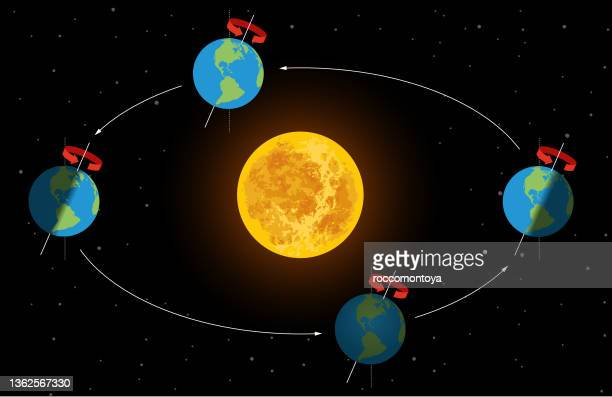
\includegraphics[width=\textwidth]{./imgs/img3.png}
\end{figure}
%Fonte: Getty Images / \href{https://www.gettyimages.com.br/fotos/earth-sun-rotation}{\emph{https://www.gettyimages.com.br/fotos/earth-sun-rotation}}

\begin{escolha}
\item Qual o nome do movimento ilustrado?

\linhas{1}
\coment{Eixo A, (EF05CI11) Translação.}

\item O movimento da rotação ocorre ao mesmo tempo que o movimento indicado na imagem?

\linhas{2}
\coment{Eixo B, (EF05CI11) Sim. Os movimentos são simultâneos, enquanto cada
rotação completa descreve um dia de aproximadamente 24 horas, as 365
rotações ocorrem durante a volta da Terra ao redor do sol.}
\end{escolha}

\num{4} Os anos terrestres duram aproximadamente 365 dias, 5 horas
e 48 minutos. O período de um ano nesse ciclo representa a movimentação
da Terra em torno do Sol, sendo assim, a volta só termina no último dia.

Por que, a cada quatro anos, tem-se um ano bissexto?

\linhas{3}
\coment{Eixo B, (EF05CI11) As horas e os minutos acumulados durante as voltas da
Terra em um ano regular totalizam, em quatro anos, a duração aproximada
de um novo dia de 24 horas. Portanto, nesse período tem-se um ano
bissexto, com um dia a mais no mês de Fevereiro.}

\num{5} São conhecidas 4 estações do ano: verão, outono, inverno e
primavera. No verão, os dias são mais iluminados e mais quentes, no
outono, caem as folhas e temperaturas, no inverno, predomina o frio, na
primavera, crescem as folhas.

\begin{escolha}
\item Como o movimento da Terra justifica as estações do ano?

\linhas{4}
\coment{Eixo B, (EF05CI11) A variação das estações do ano varia de acordo com a
posição da Terra com relação ao sol e aos hemisférios e a inclinação do
eixo de rotação. Durante o movimento de translação, ocorrem as estações
conhecidas, pois cada uma delas descreve um quarto da movimentação do
planeta em torno do sol.}

\item Como os movimentos da Terra determinam o clima em todas as regiões do planeta?

\linhas{4}
\coment{Eixo B, (EF05CI11) De acordo com a distribuição da energia solar, em
forma de luz e calor, os movimentos de rotação e translação determinam
um padrão climático para as regiões da Terra nas respectivas estações do
ano. Fatores regionais variados podem modificar o clima esperado e
característico da cada região.}
\end{escolha}

\num{6} Quando é dia em São Paulo, no Brasil, é noite em Osaka, no
Japão. Esse fenômeno pode ser representado por duas imagens comparando
os centros comerciais dessas cidades:

%COLOCAR AS IMAGENS LADO A LADO. SÃO PAULO NA ESQUERDA E OSAKA NA DIREITA
\begin{figure}[htpb!]
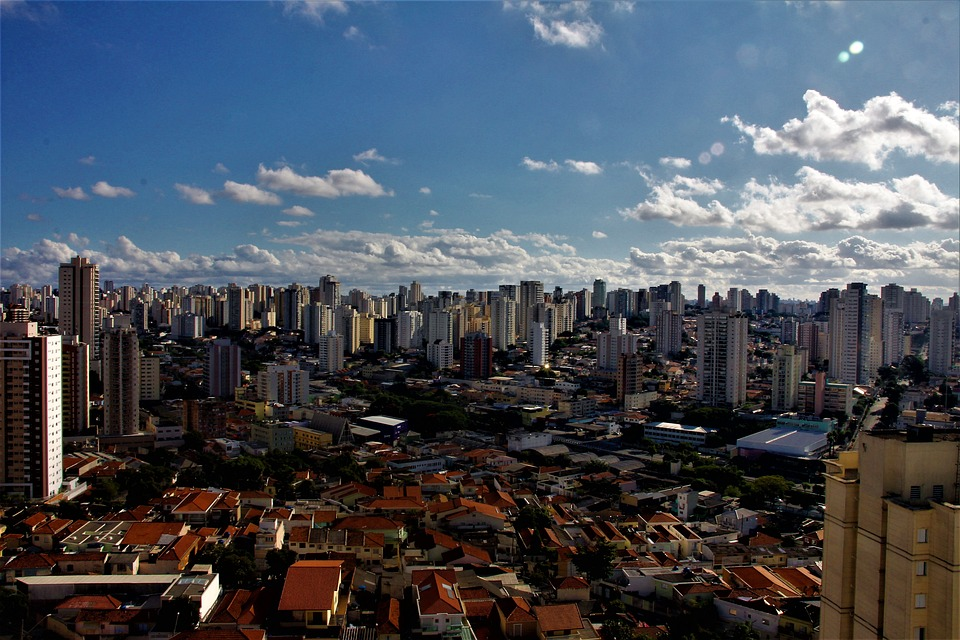
\includegraphics[width=\textwidth]{./imgs/img4.png}

\includegraphics[width=\textwidth]{./imgs/img5.png}
\end{figure}
%Imagens do Pixabay
%Imagem 1: \href{https://pixabay.com/pt/photos/s\%c3\%a3o-paulo-dia-da-sa\%c3\%bade-brasil-4958304/}{\emph{https://pixabay.com/pt/photos/s\%c3\%a3o-paulo-dia-da-sa\%c3\%bade-brasil-4958304/}}
%Imagem 2: \href{https://pixabay.com/pt/photos/jap\%c3\%a3o-osaka-pedestres-cruzando-2014616/}{\emph{https://pixabay.com/pt/photos/jap\%c3\%a3o-osaka-pedestres-cruzando-2014616/}}

Como é possível, ao mesmo tempo, que numa parte do planeta seja dia,
enquanto em outra seja noite?

\linhas{4}
\coment{Eixo B, (EF05CI11) A Terra, durante o movimento de rotação, não recebe a
luz solar da mesma maneira em todos os pontos de sua superfície
esférica. Enquanto em algumas regiões é dia, em outras, em lugares
opostos, não há incidência da luz solar. O Brasil e o Japão tem fuso
horários muito distintos por conta desse fenômeno.}

\num{7} No solstício de verão, a luz solar incide com \preencher\coment{maior}
intensidade em um dos hemisférios da terra. A principal característica
desse período é a espaço em branco maior duração dos dias.

A palavra que completa o texto é

\begin{escolha}
\item maior.

\item menor.

\item igual.

\item indiferente.
\end{escolha}

\coment{Eixo A, (EF05CI11) Alternativa a. Discuta com os alunos as diferenças
entre o solstício de verão, que ocorre em junho no hemisfério norte, e
em dezembro no hemisfério sul.}

\num{8} Relacione os itens:

\begin{multicols}{1}
1. Solstício de inverno.

2. Equinócio.

3. Rotação da lua.

4. Solstício de verão.

5. Revolução da lua.

6. Rotação da Terra.

7. Translação da lua.

\columnbreak

(\coment{4}) os dias duram mais do que as noites.

(\coment{3}) movimento da lua em torno do seu próprio eixo.

(\coment{1}) as noites duram mais do que os dias.

(\coment{7}) movimento da lua em torno do sol.

(\coment{2}) os dias e as noites possuem a mesma duração.

(\coment{6}) movimento da Terra em torno do seu próprio eixo.

(\coment{5}) giro da lua em torno da Terra.
\end{multicols}

\coment{Eixo A, (EF05CI11) (EF05CI12).}

\num{9} Marque verdadeiro (V) ou falso (F)

\begin{boxlist}
\item A lua é um satélite natural da Terra. \coment{V}

\item A luz emitida pela lua é responsável por iluminar as noites. \coment{F}

\item Rotação, revolução e translação são movimentos realizados pela lua. \coment{V}

\item Sem a lua, as noites seriam totalmente escuras. \coment{V}
\end{boxlist}

\coment{Eixo B, (EF05CI11) V, F, V, V. Afirmação falsa: a lua não é capaz de
emitir luz própria, logo, ela também não é responsável por iluminar as
noites dessa maneira.}

\num{10} Apesar de não emitir luz própria, a lua é capaz de
refletir a luz solar. Por conta desse fenômeno, conseguimos entender as
fases da lua de acordo com o que é visível na Terra. Quando a Terra está
entre a lua e o sol, temos a lua cheia, onde o satélite natural é
totalmente visível a partir da superfície terrestre. Nessa mesma fase,
ocorrem os chamados eclipses lunares.

O que são eclipses lunares?

\linhas{3}
\coment{Eixo B, (EF05CI12) São fenômenos astronômicos que ocorrem quando a
sombra do planeta Terra, posicionado entre a lua e o sol, bloqueia a
chegada de luz na superfície lunar, ou seja, quando há um alinhamento
perfeito entre Terra, sol e lua.}

\num{11} Um cientista observou as noites durante uma semana, a fim
de entender as fases da lua, e registrou as seguintes ocorrências:

\begin{longtable}[]{@{}ll@{}}
\toprule
\textbf{Dias} & \textbf{Descrição}\tabularnewline
1 e 2 & Tamanho da lua pequeno, imagem côncava e
decrescente.\tabularnewline
2 e 3 & Lua não visível.\tabularnewline
3 e 4 & Lua não visível.\tabularnewline
4 e 5 & Pequena parte da lua visível.\tabularnewline
5 e 6 & Pequena parte da lua visível.\tabularnewline
6 e 7 & Pequena parte da lua visível. Imagem côncava e
crescente.\tabularnewline
\bottomrule
\end{longtable}

Mesmo que não observasse todos os dias, a que conclusão o cientista
poderia chegar sobre as fases da lua nos três primeiros dias?

\linhas{4}
\coment{Eixo C, (EF05CI12) O cientista teria percebido que a fase da lua nos
dois primeiros dias era a lua minguante, enquanto no dia seguinte,
quando não havia lua visível, a indicação era a de lua nova. Nessa
situação, a lua se põe entre a terra e o sol, e, caso fosse um período
sinódico, se manteria nessa posição por até 8 dias.}

\conteudo{Os ciclos lunares sinódicos
duram cerca de 29,5 dias, descrevendo um mês lunar. É nesse período de
tempo que se considera um ciclo lunar completo, onde as fases da lua
duram em torno de 7 a 8 dias.

Já os ciclos lunares siderais duram aproximadamente 27,3 dias. Algumas
fases da lua podem ser incompletas, por conta dos movimentos de rotação
e revolução realizados pela lua.}

\num{12} Observe a imagem que descreve o ciclo lunar em Janeiro de 2023:

%\textbf{Calendário: 1-31/01/2023}
\begin{figure}[htpb!]
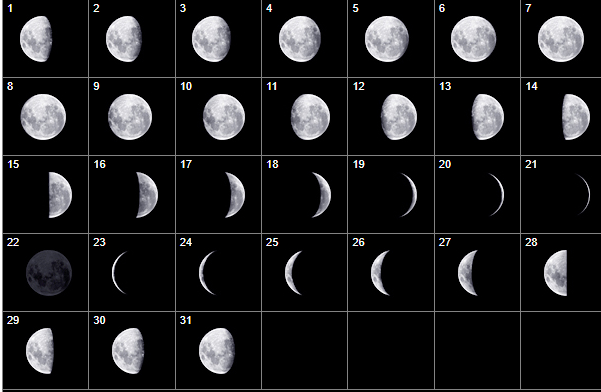
\includegraphics[width=\textwidth]{./imgs/img6.png}
\end{figure}
%\textbf{Fonte:} Moon Connection \textbf{/ \href{https://www.moonconnection.com/moon_phases_calendar.phtml}{\emph{https://www.moonconnection.com/moon\_phases\_calendar.phtml}}}

\begin{escolha}
\item Complete a tabela abaixo para cada uma das quatro fases da lua:

\begin{tabular}{|l|l|}
\hline
\textbf{Fase} & \textbf{Dia} \\ \hline
\rosa{Lua cheia} & 7 \\ \hline
Lua minguante & \begin{tabular}[c]{@{}l@{}}\rosa{Mais perceptível nos dias}\\ \rosa{13, 14, 15, 16, 17, 18, 19, 20, 21}\\ \rosa{(Qualquer um desses pode ser citado)}\end{tabular} \\ \hline
\rosa{Lua nova} & 22 \\ \hline
\rosa{Lua crescente} & 27 \\ \hline
\end{tabular}

\coment{Eixo C, (EF05CI12)}

\item Qual dos ciclos da lua pôde ser observado em janeiro de 2023?

\linhas{3}
\coment{Eixo C, (EF05CI12) Ciclo lunar sideral, pois se observam fases da lua
incompletas, como no caso da lua nova. Esse ciclo dura, aproximadamente,
27,3 dias, tendo se iniciado entre 5 e 7 de janeiro de 2023 e encerrado,
provavelmente, entre 31 de janeiro de 2023 e 02 de fevereiro de 2023.}
\end{escolha}

\colorsec{Treino}

\num{1} No mês de fevereiro, às 16h de uma tarde ensolarada no
Brasil, o Japão está mergulhado na escuridão da madrugada. Ao mesmo
tempo, tem-se o começo de um novo dia na Austrália, enquanto, nos
Estados Unidos, faz-se um dia frio.

Esse fenômeno é explicado pela

\begin{escolha}
\item irradiação do sol nas regiões da Terra.

\item diminuição das camadas de proteção solar.

\item elevação do nível d'água no hemisfério sul.

\item consolidação das mudanças climáticas na superfície terrestre.
\end{escolha}

\coment{Eixo SAEB: A.

Habilidade BNCC: (EF05CI11) Associar o movimento diário do Sol e das
demais estrelas no céu ao movimento de rotação da Terra.

a) Correto. Como a irradiação de luz solar não é uniforme em todas as
regiões da Terra, que realiza os movimentos de rotação e translação,
observam-se diferentes fuso-horários e também diferentes estações do
ano. Enquanto ocorre um dia ensolarado no Brasil, é madrugada no Japão,
alvorecer na Austrália e se vive um dia frio nos Estados Unidos;
b) Incorreto. A existência do dia e da noite em dois polos distintos da
Terra ao mesmo tempo não é explicada pela ocorrência ou falta de camadas
de proteção solar no planeta;
c) Incorreto. A elevação dos níveis d'água nos hemisférios, ainda que
representem problemas preocupantes, não explica ocorrências milenares
como a existência do dia e da noite em pontos distintos do planeta ao
mesmo tempo;
d) Incorreto. As mudanças climáticas não têm relação direta com o
fenômeno descrito, em que em pontos distintos do planeta Terra, ao mesmo
tempo, observa-se um dia quente, uma madrugada, um alvorecer e um dia
frio. Essas ocorrências são explicadas pela irradiação solar no planeta,
que muda conforme o movimento de rotação.}

\num{2} Terra e Lua estão sempre em movimento. O planeta gira em
torno do próprio eixo e completa uma rotação em torno do sol em 365
dias. A lua, além de girar em torno do próprio eixo, gira em torno da
Terra e também em torno do sol durante o ano.

Quais são os movimentos descritos no texto?

\begin{escolha}
\item Rotação terrestre, revolução terrestre, rotação lunar e translação lunar.

\item Revolução terrestre, rotação lunar, translação lunar e revolução lunar

\item Rotação terrestre, translação terrestre, rotação lunar, translação lunar e revolução lunar.

\item Rotação solar, translação terrestre, rotação lunar e revolução lunar.
\end{escolha}

\coment{Eixo SAEB: B.

Habilidade BNCC: (EF05CI12) Concluir sobre a periodicidade das fases da
Lua, com base na observação e no registro das formas aparentes da Lua no
céu ao longo de, pelo menos, dois meses.

a) Incorreto. A Terra não realiza revolução, e o texto descreve, além
dos movimentos citados, a translação terrestre, movimento de giro da
Terra em torno do sol durante 365 dias, e a revolução lunar, movimento
de giro da lua em torno da Terra durante aproximadamente 28 dias;
b) Incorreto. A Terra não realiza revolução, e os movimentos de rotação
e translação terrestre descritos no texto não foram citados;
c) Correto. Os movimentos realizados, na ordem de descrição do texto,
são rotação terrestre, translação terrestre, rotação lunar, translação
lunar e revolução lunar;
d) Incorreto. Nenhum movimento do sol foi mencionado no texto, e, além
disso, não se cita o movimento da Terra em torno do seu próprio eixo, a
rotação terrestre, e nem o movimento de giro da lua em torno do sol, a
translação lunar.}

\num{3}

\begin{quote}
É também no verão que, ao mesmo tempo em que o Sol nasce mais cedo, ele
também se põe mais tarde, o que faz com que os dias sejam mais longos. A
latitude --- a distância do local em que se está até a Linha do Equador
--- determina se um dia é mais curto ou mais longo. Quando mais próxima
uma localidade estiver desse marco, menos variações vai sofrer com as
estações do ano.

\fonte{FONTES, Ivana. \textbf{Por que o dia escurece mais tarde no verão?}.
Disponível em:
https://www.terra.com.br/byte/por-que-o-dia-escurece-mais-tarde-no-verao,1e91be126b75b69e68da0d8e27e6764bq9m733uq.html.
Acesso em: 19 fev. 2023.}
\end{quote}

O fenômeno que inicia a estação do ano citada no texto é chamado de

\begin{escolha}
\item equinócio de primavera.

\item solstício de verão.

\item solstício de inverno.

\item equinócio de outono.
\end{escolha}

\coment{Eixo SAEB: C.

Habilidade BNCC: (EF05CI11) Associar o movimento diário do Sol e das
demais estrelas no céu ao movimento de rotação da Terra.

a) Incorreto. O equinócio de primavera representa o período de fim do
inverno e começo da primavera, ou seja, nessas datas, a incidência da
luz solar é maior na região equatorial da Terra, fazendo com que os dias
e as noites tenham durações iguais;
b) Correto. No solstício de verão, há maior incidência da luz solar em
um dos hemisférios da terra --- norte, em junho e sul, em dezembro.
Nesse período, inicia-se o verão, quanto os dias duram mais do que as
noites;
c) Incorreto. No solstício de inverno, há menor incidência da luz solar
em um dos hemisférios da terra --- norte, em dezembro e sul, em junho.
Nesse período, inicia-se o inverno, quando as noites duram mais do que
os dias;
d) Incorreto. O equinócio de outono representa o período de fim do verão
e começo do outono, ou seja, nessas datas, a incidência da luz solar é
maior na região equatorial da Terra, fazendo com que os dias e as noites
tenham durações iguais.}

\chapter{Simulado 1}

\num{1} O polígono das secas é uma região que compreende os estados
brasileiros de Alagoas, Bahia, Ceará, Minas Gerais, Paraíba, Pernambuco,
Piauí, Rio Grande do Norte e Sergipe. Nessas localidades, os
trabalhadores rurais relatam que são comuns os longos períodos de seca.
Sem rios abundantes, as águas locais são encontradas em temperatura
menor que o normal, o que dificulta a evaporação. Toda a produção
agrícola é adaptada para a época de chuva, mais comum em fevereiro.

Uma das explicações para a falta de chuvas da região pode ser

\begin{escolha}
\item o acúmulo de erros de gestão pública.

\item o uso indiscriminado da água.

\item a evaporação acelerada das águas locais.

\item a baixa umidade do ar.
\end{escolha}

\coment{Eixo SAEB: C.

Habilidade BNCC: (EF05CI02) Aplicar os conhecimentos sobre as mudanças
de estado físico da água para explicar o ciclo hidrológico e analisar
suas implicações na agricultura, no clima, na geração de energia
elétrica, no provimento de água potável e no equilíbrio dos ecossistemas
regionais (ou locais).

a) Incorreto. Apesar da gestão pública poder lidar com o problema, de
maneira a mitigar os potenciais danos, as características do polígono da
seca são naturais, decorrentes do ciclo hidrológico da água nesta
região;
b) Incorreto. O uso indiscriminado da água, neste caso, não explica a
falta de chuvas em toda a região de estados com diferentes populações e
costumes;
c) Incorreto. A evaporação das águas locais é lenta, pois estas tem por
característica uma temperatura menor que as de outras localidades. Sendo
assim, a evaporação se torna mais difícil;
d) Correto. A umidade do ar é muito baixa na região, graças à ausência
de rios abundantes e da característica das águas locais de possuir
temperatura mais baixa. Sendo assim, há menor disponibilidade de água
evaporada para o ciclo hidrológico da água, e, portanto, longos períodos
de seca são registrados.}

\num{2} Nos pulmões, acontece o processo conhecido como hematose. O
gás oxigênio inspirado é incorporado à corrente sanguínea pelos
alvéolos, enquanto o gás carbônico é removido e eliminado na expiração.
Esse processo é fundamental para a produção de energia no organismo,
pois o oxigênio participa de etapas da nutrição do organismo, como na
quebra de nutrientes para geração de energia.

O processo que acontece nos pulmões também pode ser chamado de

\begin{escolha}
\item nutrição.

\item troca gasosa.

\item respiração celular.

\item filtração pulmonar.
\end{escolha}

\coment{Eixo SAEB: B.

Habilidade BNCC: (EF05CI06) Selecionar argumentos que justifiquem por
que os sistemas digestório e respiratório são considerados
corresponsáveis pelo processo de nutrição do organismo, com base na
identificação das funções desses sistemas.

a) Incorreto. A nutrição diz respeito às escolhas de fontes de
nutrientes, geralmente relacionada com a alimentação, e não explica o
processo de troca de gases que acontece nos pulmões;
b) Correto. A hematose é um processo de troca gasosa, em que há infusão
de gás oxigênio inspirado no sangue, ao passo em que o gás carbônico é
eliminado do corpo por meio da expiração. Os gases são, assim, trocados
o tempo todo durante o processo respiratório, que atua de maneira
conjunta com o processo digestório;
c) Incorreto. A respiração celular é um processo de obtenção de energia
baseado na oxidação, mas não ocorre nos pulmões e nem pode ser chamada
de hematose. É uma etapa distinta na produção de energia;
d) Incorreto. A filtração pulmonar não pode ser descrita pela troca
entre gases no pulmão. É um conceito genérico, que não leva em
consideração o processo inspiratório e expiratório.}

\num{3} Uma criança, ao olhar para a lua pela janela do quarto,
observou a forte iluminação do corpo celeste. Ela concluiu, então, que
as noites são iluminadas pela luz irradiada pela lua, mas foi
repreendida ao dizer isso para a mãe, que a corrigiu e prometeu
observar, junto a ela, as fases da lua a cada semana.

A criança estava errada em sua observação, pois

\begin{escolha}
\item as noites sem a lua seriam mais claras.

\item a lua não possui iluminação própria.

\item o sol é um satélite natural mais poderoso.

\item a visualização da lua sem um telescópio é enganosa.
\end{escolha}

\coment{Eixo SAEB: A.

Habilidade BNCC: (EF05CI12) Concluir sobre a periodicidade das fases da
Lua, com base na observação e no registro das formas aparentes da Lua no
céu ao longo de, pelo menos, dois meses.

a) Incorreto. Sem a lua, não se pode prever como seriam os dias ou as
noites, pois haveria implicações acerca da posição e iluminação da
Terra;
b) Correto. A luz da lua é apenas uma reflexão da luz solar;
c) Incorreto. O sol é uma estrela, não um satélite natural, ou seja, não
tem a órbita atrelada a um planeta;
d) Incorreto. A lua pode ser vista da superfície terrestre sem um
telescópio em suas quatro fases, embora a visualização com um telescópio
forneça detalhes mais próximos que a observação a olho nu.}

\chapter{Simulado 2}

\num{1} O coração, sangue e vasos sanguíneos compõem a estrutura do
sistema circulatório. Em conjunção com outros sistemas do organismo, o
sistema circulatório participa da nutrição das células do corpo humano,
transportando nutrientes para músculos e órgãos.

Esse sistema também tem por função a

\begin{escolha}
\item produção de gases.

\item eliminação de toxinas.

\item maturação de nutrientes.

\item digestão de alimentos.
\end{escolha}

\coment{Eixo SAEB: B.

Habilidade BNCC: (EF05CI06) Selecionar argumentos que justifiquem por
que os sistemas digestório e respiratório são considerados
corresponsáveis pelo processo de nutrição do organismo, com base na
identificação das funções desses sistemas.

a) Incorreto. O sistema circulatório não tem por função a produção
gasosa, e sim o transporte do gás oxigênio incorporado à corrente
sanguínea para as estruturas do corpo humano;
b) Correto. Além de transportar nutrientes e gás oxigênio para os
tecidos do corpo humano, o sistema circulatório encaminha as substâncias
tóxicas, como as toxinas, para a eliminação;
c) Incorreto. A maturação de nutrientes não acontece no sistema
circulatório, responsável pelo encaminhamento desses após fases dos
processos respiratório e digestivo;
d) Incorreto. A digestão de alimentos é função do sistema digestório,
capaz de quebrá-los em diversos órgãos para a absorção de diferentes
partes de um alimento. O sistema circulatório atua no transporte dessas
células concentradas em nutrientes para as extremidades do corpo humano.}

\num{2} Um relatório de especialistas descreveu que, às margens de
um rio brasileiro, há pouca concentração vegetal, e uma extensa
deterioração do solo, tornando-o improdutivo. Além disso, o acúmulo de
lixo na região é muito grande. Eles concluíram que a área foi afetada
pela atividade humana, e entregaram uma série de medidas para as
autoridades, visando evitar maiores problemas.

\begin{longtable}[]{@{}ll@{}}
\toprule
\textbf{Medida} & \textbf{Justificativa}\tabularnewline
Cultivo de plantas leguminosas. & Adubar o solo
empobrecido.\tabularnewline
Instalação de barreiras de contenção. & Impedir o acúmulo de detritos no
rio.\tabularnewline
Remoção do lixo acumulado na região. & Prevenir o transporte do lixo até
o rio.\tabularnewline
Plantio de árvores no solo recuperado. & Reflorestar o entorno do
rio.\tabularnewline
\bottomrule
\end{longtable}

Tais medidas buscam prevenir o processo de

\begin{escolha}
\item ressecamento de nascentes.

\item cruzamento de correntes oceânicas.

\item escoamento das águas.

\item assoreamento do rio.
\end{escolha}

\coment{Eixo SAEB: C.

Habilidade BNCC: (EF05CI03) Selecionar argumentos que justifiquem a
importância da cobertura vegetal para a manutenção do ciclo da água, a
conservação dos solos, dos cursos de água e da qualidade do ar
atmosférico.

a) Incorreto. O ressecamento de nascentes pode ocorrer por falta de água
nos lençóis freáticos. Os problemas apontados e as medidas de correção
não buscam combater esse problema;
b) Incorreto. Dentre os problemas apontados e soluções pretendidas, não
há relação com o cruzamento de correntes oceânicas distintas, que ocorre
com a movimentação de grandes quantidades de água em oceanos e mares;
c) Incorreto. O escoamento regular da água de um rio não representa um
problema a ser solucionado, sendo influenciado por fatores como o regime
de chuvas e o ciclo hidrológico de determinada região;
d) Correto. Ao tratar o solo erodido, replantar uma estrutura vegetal,
reflorestar o entorno do rio e recolher o lixo depositado, os
especialistas buscam prevenir a intensificação do assoreamento do rio
pela atividade humana, processo que pode atrapalhar os cursos d'água,
causar inundações e morte de espécies marinhas.}

\num{3} Em 21/12/2022, o Brasil teve o dia mais longo e a noite
mais curta do ano. Esse período marcou a passagem da primavera para o
verão no país, graças à maior incidência de luz do sol no hemisfério sul
e à inclinação do planeta Terra. Esse fenômeno é conhecido como
solstício de verão.

No hemisfério norte, qual estação do ano se iniciou no mesmo dia?

\begin{escolha}
\item Primavera.

\item Outono.

\item Verão.

\item Inverno.
\end{escolha}

\coment{Eixo SAEB: B.

Habilidade BNCC: (EF05CI11) Associar o movimento diário do Sol e das
demais estrelas no céu ao movimento de rotação da Terra.

a) Incorreto. Se a primavera estava terminando no hemisfério sul, o
oposto acontecia no hemisfério norte. Portanto, terminava o outono para
se iniciar o inverno;
b) Incorreto. No hemisfério norte, o outono terminava para dar lugar ao
inverno;
c) Incorreto. O verão iniciou no hemisfério sul, portanto, não poderia
também iniciar no hemisfério oposto;
d) Correto. No hemisfério norte, no mesmo período do ano, tem-se início
o inverno, graças ao movimento de rotação da terra e da inclinação do
planeta, fazendo com que haja menor incidência da luz solar na região
oposta ao hemisfério sul.}

\chapter{Simulado 3}

\num{1} No estômago, o alimento é envolvido pelo suco gástrico.
Forma-se, assim, uma massa de bolo alimentar chamada quimo. Quando chega
ao intestino delgado, o quimo passa por ações de várias substâncias, que
aproveitam os nutrientes necessários, como o amido e as proteínas, e,
então, passa a ser chamado de quilo.

O texto descreve etapas do processo de

\begin{escolha}
\item digestão.

\item alimentação.

\item hidratação.

\item evacuação.
\end{escolha}

\coment{Eixo SAEB: A.

Habilidade BNCC: (EF05CI06) Selecionar argumentos que justifiquem por
que os sistemas digestório e respiratório são considerados
corresponsáveis pelo processo de nutrição do organismo, com base na
identificação das funções desses sistemas.

a) Correto. A produção do quimo e do quilo, além dos órgãos mencionados,
é descrita no processo de digestão;
b) Incorreto. A alimentação vem antes da digestão e é, costumeiramente,
uma ação mecânica que acontece a partir da boca. É dela que advém os
nutrientes a serem digeridos e processados no organismo;
c) Incorreto. O processo de hidratação do organismo ocorre com a
ingestão de água, e, portanto, não é descrito nas etapas de produção de
quimo e quilo;
d) Incorreto. A evacuação é a etapa de eliminação das fezes do
organismo, que são o produto final restante de todas as etapas da
digestão, sendo assim, é apenas mais uma etapa do processo de digestão.}

\num{2} A densidade nutricional de um alimento é uma classificação
que separa as calorias consumidas em cheias ou vazias. As calorias
cheias são as que fornecem quantidades de vitaminas, fibras, gorduras e
proteínas em equilíbrio, enquanto as vazias apresentam um número elevado
de açúcares e gorduras.

Alimentos com menor densidade nutricional apresentam calorias vazias
pois

\begin{escolha}
\item são alimentos com menor teor calórico.

\item são essenciais para qualquer dieta.

\item são uma fonte pobre de nutrientes.

\item são menos ofensivos ao organismo.
\end{escolha}

\coment{Eixo SAEB: C.

Habilidade BNCC: (EF05CI08) Organizar um cardápio equilibrado com base
nas características dos grupos alimentares (nutrientes e calorias) e nas
necessidades individuais (atividades realizadas, idade, sexo etc.) para
a manutenção da saúde do organismo.

a) Incorreto. Alimentos ricos em gorduras e açúcares representam,
geralmente, maior teor calórico que outros, embora somente essa
informação não seja usada para classificação em calorias vazias ou
cheias;
b) Incorreto. A alimentação com fontes pobres de calorias não é
essencial para as dietas dos seres humanos, sejam elas quais forem, e
deve ser realizada de maneira consciente e sem excessos;
c) Correto. Como são compostas majoritariamente por gorduras e açúcares,
as calorias vazias são pobres em demais nutrientes como vitaminas,
fibras e proteínas;
d) Incorreto. Calorias vazias podem, quando ingeridas em excesso, causar
doenças como o câncer e a diabetes. Não são, portanto, menos ofensivas
ao organismo que as calorias cheias.}

\num{3} Ao estudar as fases da lua, um pesquisador observou o céu
todas as noites, a fim de anotar informações sobre a visibilidade do
satélite natural da Terra. Ele registrou as anotações numa tabela:

\begin{longtable}[]{@{}ll@{}}
\toprule
\textbf{Semana} & \textbf{Fase da lua}\tabularnewline
1 & Minguante\tabularnewline
2 & Nova\tabularnewline
3 & Crescente\tabularnewline
4 & Cheia\tabularnewline
\bottomrule
\end{longtable}

Com base nessas informações, observou que se tratava de um ciclo lunar
sinódico, em cada fase dura entre 7 e 8 dias.

No meio da semana 5, qual será a fase da lua?

\begin{escolha}
\item Cheia.

\item Nova.

\item Crescente.

\item Minguante.
\end{escolha}

\coment{Eixo SAEB: B.

Habilidade BNCC: (EF05CI12) Concluir sobre a periodicidade das fases da
Lua, com base na observação e no registro das formas aparentes da Lua no
céu ao longo de, pelo menos, dois meses.

a) Incorreto. A lua cheia acontece na semana 4, portanto, num ciclo
lunar sinódico em meados da semana 5 ocorrerá a fase seguinte, que é a
lua minguante;
b) Incorreto. A lua nova não pode ocorrer logo após a lua cheia,
necessitando, num ciclo lunar sinódico, da transição que passa pela
ocorrência da lua minguante;
c) Incorreto. A lua cheia não pode dar lugar à lua crescente, que é a
fase da lua que a antecede. Isso só poderia ocorrer caso a fase anterior
fosse a lua nova;
d) Correto. Como se trata de um ciclo lunar sinódico, ou seja, completo,
a fase seguinte que se espera observar no meio da semana é a lua
minguante.}

\chapter{Simulado 4}

\num{1} Em dias quentes de verão, observam-se altas temperaturas
nas manhãs e tardes, e fortes chuvas nas noites e nos dias seguintes. A
explicação desse fenômeno reside no fato da umidade do ar se elevar
nessa época do ano em comparação com outras estações.

O ar se torna mais úmido nesse período pois

\begin{escolha}
\item a evaporação e a evapotranspiração acontecem com maior intensidade.

\item a intensidade da luz solar impede chuvas mais frequentes.

\item o acúmulo de vapor de água nas nuvens é incomum em dias quentes.

\item o sol participa da formação de gotículas de água antes da chuva.
\end{escolha}

\coment{Eixo SAEB: C.

Habilidade BNCC: (EF05CI02) Aplicar os conhecimentos sobre as mudanças
de estado físico da água para explicar o ciclo hidrológico e analisar
suas implicações na agricultura, no clima, na geração de energia
elétrica, no provimento de água potável e no equilíbrio dos ecossistemas
regionais (ou locais).

a) Correto. Em dias mais quentes, há a intensificação de fenômenos
essenciais para o aumento do regime de chuvas: a evaporação de águas de
oceanos, rios e solos e a evapotranspiração de plantas. Com isso, o ar
se torna mais úmido e as chuvas caem com maior frequência;
b) Incorreto. A luz solar mais intensa pode aquecer mais as fontes de
água a ser vaporizada, mas não consegue impedir a frequência de chuvas,
que é relatada no texto como mais frequente no verão;
c) Incorreto. Em dias quentes, é comum que se observe um considerável
aumento na precipitação das nuvens;
d) Incorreto. O sol não participa da formação de gotículas de chuva
diretamente, e sim na vaporização da água que, ao chegar nas nuvens, se
agrega para formar gotículas.}

\num{2} Pequenos agricultores decidiram substituir as bombas d'água
que utilizavam água tratada para a irrigação das plantações. No lugar de
utilizar a água que vinha das companhias fornecedoras, criaram um tanque
para depositar água residual proveniente de atividades diárias que
desperdiçam água, goteiras e outras atividades agrícolas, como a própria
irrigação. Algumas espécies vegetais capazes de filtrar as impurezas da
água também foram utilizadas num pequeno circuito de tratamento.

A reutilização da água, nessas condições, é possível pois

\begin{escolha}
\item as plantações podem sobreviver com qualquer tipo de água.

\item o pequeno agricultor não trabalha com grandes plantações.

\item a irrigação representa o uso da água para um fim não-potável.

\item a água de reuso é mais importante para o crescimento de vegetais.
\end{escolha}

\coment{Eixo SAEB: B.

Habilidade BNCC: (EF05CI04) Identificar os principais usos da água e de
outros materiais nas atividades cotidianas para discutir e propor formas
sustentáveis de utilização desses recursos.

a) Incorreto. As plantações não sobrevivem com o uso de resíduos de água
com toxinas e contaminantes, por isso nem todo tipo de água pode ser
reutilizada;
b) Incorreto. Apesar de pequenos agricultores lidarem com um volume de
plantações muito menor que o de grandes empresas, não é esse o fato que
justifica a reutilização da água, que também deve ser feita em escala
industrial;
c) Correto. Atividades como a irrigação consomem a água para fins
não-potáveis. Nessas situações, pode-se reutilizar águas residuais;
d) Incorreto. A água de reuso não desempenha papel fundamental e
decisivo no crescimento de vegetais, pois não apresenta componentes que
possam acelerar esse processo.}

\num{3} A digestão dos alimentos começa na boca, e o sistema
digestório é capaz de selecionar os nutrientes necessários para o
funcionamento do organismo e a produção de energia, dividindo os
alimentos em partículas menores. O oxigênio, inalado na inspiração,
participa da produção de energia no aproveitamento dos nutrientes,
enquanto o coração bombeia o sangue concentrado nos nutrientes divididos
para todos os tecidos do organismo humano.

A ação dos sistemas digestório, respiratório e circulatório após a
alimentação demonstra que

\begin{escolha}
\item o sistema respiratório é menos importante no processo de nutrição.

\item os sistemas atuam em conjunto no organismo humano.

\item a produção de energia poderia ser realizada somente pelo estômago.

\item o organismo pode sobreviver sem alimentos por muito tempo
\end{escolha}

\coment{Eixo SAEB: B.

Habilidade BNCC: (EF05CI06) Selecionar argumentos que justifiquem por
que os sistemas digestório e respiratório são considerados
corresponsáveis pelo processo de nutrição do organismo, com base na
identificação das funções desses sistemas. e (EF05CI07) Justificar a
relação entre o funcionamento do sistema circulatório, a distribuição
dos nutrientes pelo organismo e a eliminação dos resíduos produzidos.

a) Incorreto. Todos os três sistemas possuem papéis importantes e
fundamentais no processo de nutrição do organismo, sendo indispensáveis
para a produção de energia e manutenção da vida;
b) Correto. A ação conjunta dos sistemas garante a digestão, seleção de
nutrientes, produção de energia na divisão dos nutrientes, transporte e
fixação nos tecidos do corpo humano;
c) Incorreto. O sistema digestório é composto por diversos órgãos, e a
etapa da produção de energia precisa do oxigênio inspirado no sistema
respiratório e transportado no sangue pelo sistema circulatório;
d) Incorreto. Apesar de possuir reservas energéticas e de gordura, a
ação dos sistemas demonstra que eles funcionam em conjunto, mas não são
capazes de manter a sobrevivência saudável de um ser humano sem a
alimentação.}

%REFERÊNCIAS

%DÂNGELO, J. G.; FATTINI, C. A. Anatomia humana sistêmica e segmentar. 2a
%ed. Rio de Janeiro: Atheneu, 2011.
%
%FERREIRA, P. F.; LEITE, C. A FORMA E OS MOVIMENTOS DA TERRA: PERCEPÇÕES
%DE PROFESSORES ACERCA DAS RELAÇÕES ENTRE OBSERVAÇÃO COTIDIANA E OS
%MODELOS CIENTÍFICOS. \textbf{Revista Latino-Americana de Educação em
%Astronomia - RELEA}, n. 19, p. 123-146, 2015
%
%GONÇALVES, P. C. DA S.; BRETONES, P. S.. O ensino sobre a Lua e suas
%fases: uma proposta observacional para os Anos Iniciais do Ensino
%Fundamental. \textbf{Ensaio Pesquisa em Educação em Ciências (Belo
%Horizonte)}, v. 23, n. Ens. Pesqui. Educ. Ciênc. (Belo Horizonte), 2021.
%
%HORNIK, G. G.; HENRIQUE, A.; HORNIK, E. N. H\textsubscript{2}O - O Ciclo
%da Vida. Alfenas: Independente, 2016.
%
%MIRANDA, R. A. C.; OLIVEIRA, M. V. S.; SILVA, D. F. CICLO HIDROLÓGICO
%PLANETÁRIO: abordagens e Conceitos. \textbf{Geo UERJ}, Rio de Janeiro -
%RJ, ano 12, v. 1, n. 21, 2010.
%
%TONEL, A. P.; MARRANGHELLO, G. F.. O movimento aparente da Lua. Revista
%Brasileira de Ensino de Física, v. 35, n. \textbf{Rev. Bras. Ensino
%Fís.}, 2013 35(2), abr. 2013.
